\documentclass[13pt,aspectratio=169]{beamer}

\usepackage[utf8]{inputenc}
\usepackage{tikz}
\usetikzlibrary {arrows.meta}
\usepackage{amssymb}
\usepackage{amsmath}
\usepackage{mathrsfs}
\usepackage{bbm}
\usepackage{multirow}

\usetheme{Madrid}
\usecolortheme{seahorse}

\title{Unbiased VICReg}
\author{S.~Bezyazichniy, \\E.~Serov, \\D.~Ivanov, \\P.~Lisov, \\N.~Groza}
\institute{MIPT}
\date{October 2, 2024}

\begin{document}

\begin{frame}
  \titlepage
\end{frame}

\begin{frame}
	\frametitle{Contents}
	\tableofcontents
\end{frame}

\section{Basic SSL Idea}
\begin{frame}
  \frametitle{Preventing Collapse in Self-Supervised Learning}
  \begin{itemize}
    \item \textbf{Self-Supervised Learning (SSL)} has made
      significant progress, allowing models to learn without
      labeled data by maximizing agreement between embeddings
      of different views of the same image or other object.
    \item \textbf{Main Challenge:} In joint embedding architectures
      models often \textit{collapse} producing constant, non-informative
      embeddings.
  \end{itemize}

  \begin{figure}
      \begin{center}
  	    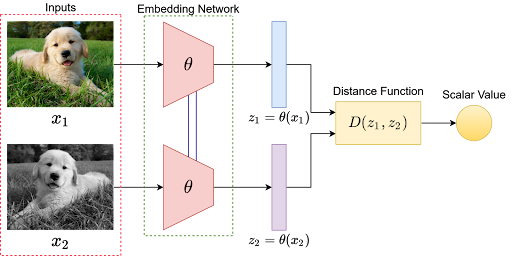
\includegraphics[width=0.65\textwidth]{imgs/je_architecture.png}
      \end{center}
  \end{figure}
  
\end{frame}

\section{SimCLR}
\begin{frame}
  \frametitle{Simple Framework for Contrastive Learning of Visual Representations}

  \begin{columns}
    \begin{column}{0.5\textwidth}
      \begin{enumerate}
	\item \textbf{Augmentation:} generate two correlated views from given data
	  using random cropping, resizing, horizontal flipping, colour distortion, grey scaling 
	  and/or Gaussian blur.
	\item \textbf{Encoder:} extract representation vectors from augmented data.
	\item \textbf{Projection head:} map representations to the embedding space where
	  contrastive loss is applied. This small neural network with one hidden layer 
	  improves the quality of learned representations.
      \end{enumerate}
    \end{column}

    \begin{column}{0.5\textwidth}
      \usebeamercolor{block body}
      \begin{tikzpicture}[scale=0.8]
	\filldraw[fill={block body.bg}, draw=fg] (0,10) node (x) {$x$} circle (0.3);
	\filldraw[fill={block body.bg}, draw=fg] (-3,9) node (xi) {$\widetilde{x_i}$} circle (0.3);
	\filldraw[fill={block body.bg}, draw=fg] (3,9) node (xj) {$\widetilde{x_j}$} circle (0.3);
	\filldraw[fill={block body.bg}, draw=fg] (-3,7) node (hi) {$h_i$} circle (0.3);
	\filldraw[fill={block body.bg}, draw=fg] (3,7) node (hj) {$h_j$} circle (0.3);
	\filldraw[fill={block body.bg}, draw=fg] (-3,5) node (zi) {$z_i$} circle (0.3);
	\filldraw[fill={block body.bg}, draw=fg] (3,5) node (zj) {$z_j$} circle (0.3);

	\draw[-{Latex}] (x) -- (xi) node[midway, above] {$t \thicksim T$};
	\draw[-{Latex}] (x) -- (xj) node[midway, above] {$t' \thicksim T$};
	\draw[-{Latex}] (xi) -- (hi) node [midway, left] {$f(\cdot)$};
	\draw[-{Latex}] (xj) -- (hj) node [midway, right] {$f(\cdot)$};
	\draw[-{Latex}] (hi) -- (zi) node [midway, left] {$g(\cdot)$};
	\draw[-{Latex}] (hj) -- (zj) node [midway, right] {$g(\cdot)$};
	\draw[<->] (hi) -- (hj) node [midway, above] {Representation};
	\draw[<->] (zi) -- (zj) node [midway, above] {Maximize agreement};

      \end{tikzpicture}
       
      \begin{figure}
	  \begin{center}
		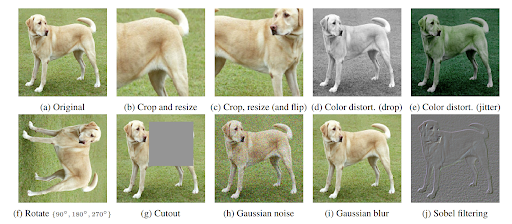
\includegraphics[width=0.65\textwidth]{imgs/simclr_pipeline.png}
	  \end{center}
      \end{figure}
    \end{column}
  \end{columns}
\end{frame}

\begin{frame}
  \frametitle{Contrastive Loss}
  SimCLR aims to learn representations by \textit{maximizing} 
  agreement between differently augmented views of the same 
  image (positive pairs) and \textit{minimizing} it for different images 
  (negative pairs).

  \begin{equation*}
    \text{sim}(u, v) = \frac{u^{\intercal} v}{\| u \| \cdot \| v \|}
  \end{equation*}
  \begin{equation*}
    \tau\text{~--- hyperparameter}
  \end{equation*}
  \begin{equation*}
    \mathfrak{l}_{i,j} = -\log \frac{\exp { \frac{\text{sim}(z_i, z_j)}{\tau} }}{\sum_{k=1}^{2N} \mathbbm{I}_{(k \neq i)} \exp{\frac{\text{sim}(z_i, z_k)}{\tau}}}
  \end{equation*}

\end{frame}

\begin{frame}
  \frametitle{Batch Size and Learning Rate Scaling}
  \begin{figure}
  	\begin{center}
  		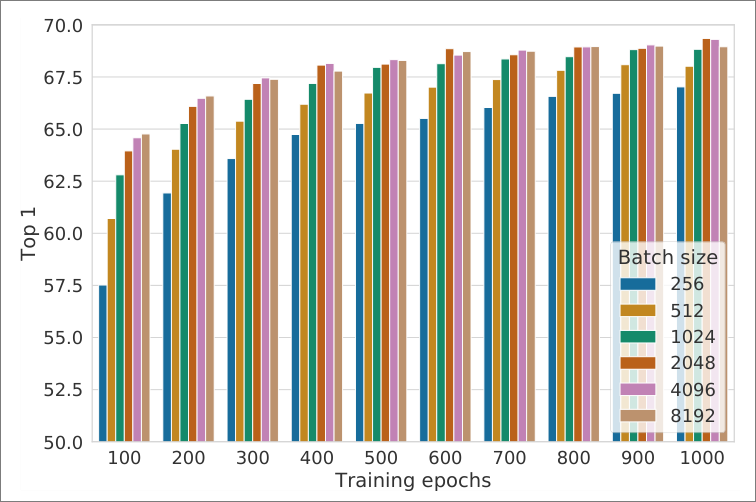
\includegraphics[height=6cm]{imgs/batch_size_simclr.png}
  	\end{center}
	\caption{Linear evaluation models (ResNet-50)
	trained with different batch sizes and epochs. Each
	bar is a single run from scratch}
  \end{figure}
  
\end{frame}

\section{VICReg}
\begin{frame}
  \frametitle{VICReg}
  \begin{figure}
  	\begin{center}
  		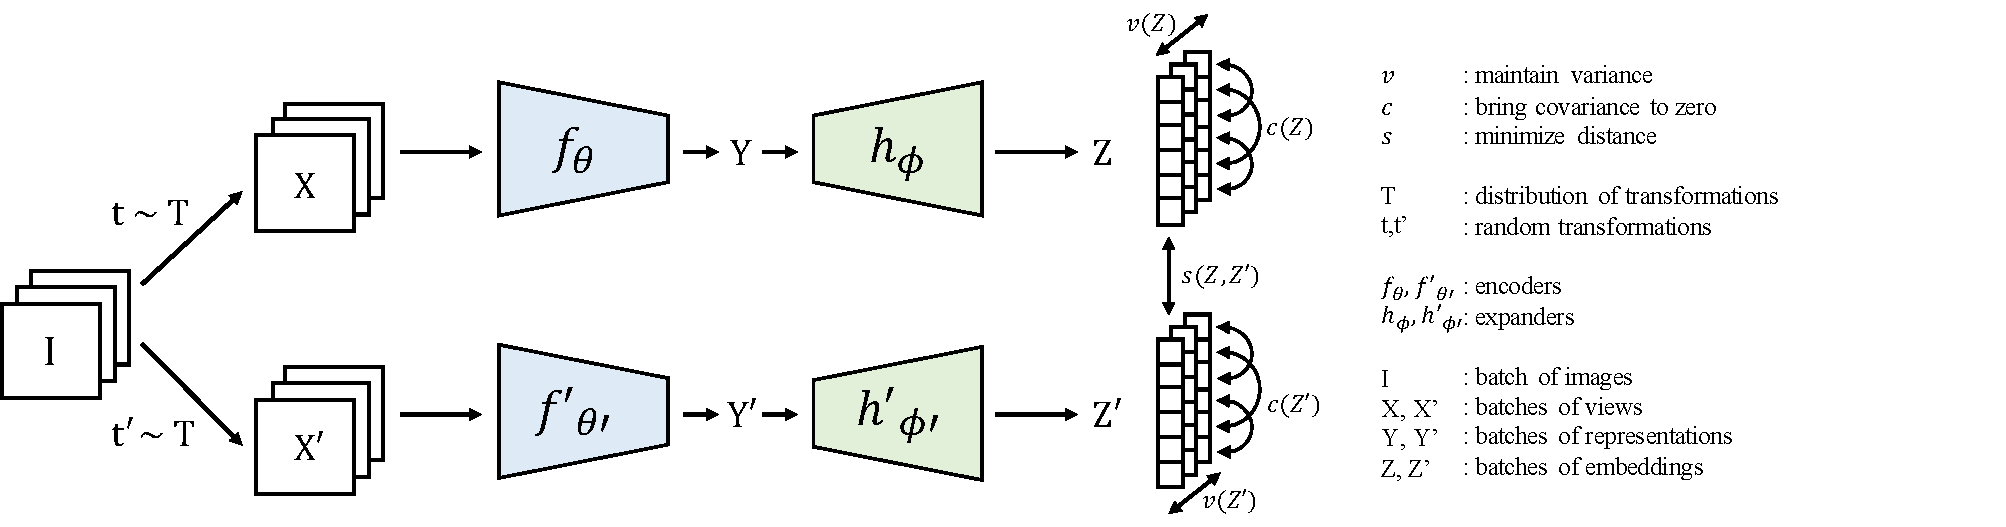
\includegraphics[width=0.95\textwidth]{imgs/vicreg_architecture.pdf}
  	\end{center}
  \end{figure}
  
\end{frame}

\begin{frame}
  \frametitle{VIC}

  Consider $Z = (z_1, \dots, z_n)$ and $Z' = (z'_1, \dots, z'_n)$ be the two
  batches composed of $n$ vectors of dimension $d$.

  \begin{itemize}
    \item \textbf{Invariance:}
      \begin{equation*}
	s(Z, Z') = \frac{1}{n}\sum_{i=1}^n \| z_i - z'_i \|_2^2.
      \end{equation*}

    \item \textbf{Variance:}
      \begin{equation*}
	v(Z) = \frac{1}{d} \sum_{i=1}^d \max (0, \gamma - \sqrt{\mathbbm{V}z^j + \varepsilon}),
      \end{equation*}
      where $\gamma$~--- minimal standard deviation,
      $\varepsilon$~--- small scalar preventing numerical instabilities.

    \item \textbf{Covariance:}
      \begin{equation*}
	c(Z) = \frac{1}{d} \sum_{i=1}^d | C(Z) |_{(i,j)}^2\text{, where }C(Z) = \frac{1}{n-1} \sum_{i=1}^n (z_i - z)(z_i - z)^{\intercal}.
      \end{equation*}
  \end{itemize}
\end{frame}

\begin{frame}
  \frametitle{Reg}
  The loss function over batch is
  \begin{equation*}
    \mathfrak{l}(Z,Z') = \lambda s(Z,Z') + \mu(v(Z) + v(Z')) + \nu(c(Z) + c(Z'))\text{, where }\lambda = \mu > \nu\text{ in most cases}.
  \end{equation*}

  The overall objective function on all images over dataset $\mathfrak{D}$ is
  \begin{equation*}
    \mathfrak{L} = \sum_{I \in \mathfrak{D}} \sum_{t, t' \thicksim T} \mathfrak{l}(g(f(t(I))), g(f(t'(I))).
  \end{equation*}

  \begin{columns}
    \begin{column}{0.7\textwidth}
      Model's performance is less dependent on large batch sizes 
      because it does not rely on negative samples. Instead, it focuses on 
      regularizing the variance, invariance and covariance of the learned embeddings, 
      making it more flexible and effective even with smaller batch sizes. 
    \end{column}
    \begin{column}{0.4\textwidth}
      \begin{tikzpicture}[scale=0.8]
	\filldraw[fill=bg, draw=bg] (1,-2) circle (0.35) node (z1) {$Z'$};
	\filldraw[fill={block body.bg}, draw=fg] (4,-2) circle (0.35) node (c1) {$c$};
	\filldraw[fill={block body.bg}, draw=fg] (3,-1) circle (0.35) node (v1) {$v$};
	\filldraw[fill=bg, draw=bg] (1,2) circle (0.35) node (z) {$Z$};
	\filldraw[fill={block body.bg}, draw=fg] (4,2) circle (0.35) node (c) {$c$};
	\filldraw[fill={block body.bg}, draw=fg] (3,1) circle (0.35) node (v) {$v$};
	\filldraw[fill={block body.bg}, draw=fg] (2,0) circle (0.35) node (s) {$s$};
	\filldraw[fill={block body.bg}, draw=fg] (6,0) circle (0.35) node (l) {$\mathfrak{l}$};

	\draw[-{Latex}] (z) -- (c);
	\draw[-{Latex}] (z) -- (v);
	\draw[-{Latex}] (z) -- (s);
	\draw[-{Latex}] (v) -- (l) node[midway, above] {$\mu$};
	\draw[-{Latex}] (c) -- (l) node[midway, above] {$\nu$};
	\draw[-{Latex}] (z1) -- (c1);
	\draw[-{Latex}] (z1) -- (v1);
	\draw[-{Latex}] (z1) -- (s);
	\draw[-{Latex}] (v1) -- (l) node[midway, below] {$\mu$};
	\draw[-{Latex}] (c1) -- (l) node[midway, below] {$\nu$};
	\draw[-{Latex}] (s) -- (l) node[midway, above] {$\lambda$};
      \end{tikzpicture}
    \end{column}
  \end{columns}

\end{frame}

\section{SimCLR vs VICReg}
\begin{frame}
  \frametitle{SimCLR vs VICReg}

  \begin{figure}
    \centering
    \begin{tabular}{| c | c | c | c | c | c |}
      \hline
      \multirow{2}{*}{Method} & \multicolumn{5}{|c|}{Batch size} \\
      \cline{2-6}
      & $256$ & $512$ & $1024$ & $2048$ & $4092$ \\
      \hline
      SimCLR & $57.5$ & $60.7$ & $62.8$ & $64.0$ & $64.6$ \\
      \hline
      VICReg & $67.9$ & $68.2$ & $68.3$ & $68.6$ & $67.8$ \\
      \hline
    \end{tabular}
    \caption{Impact of batch size to Top-1 accuracy after 100 epochs on ImageNet.}
  \end{figure}
\end{frame}

\section{Unbiased VICReg}
\begin{frame}
  \frametitle{Unbiased VICReg}
  \textbf{Assumption.} By making the VICReg gradient unbiased,
  we can eliminate the dependency on batch size, 
  leading to more stable training with smaller batches.
  To accomplish this, we need to identify an unbiased estimator 
  for the following loss function:

  \begin{equation*}
    \mathfrak{L} = \lambda \underset{X \thicksim \mathfrak{D}, t, t' \thicksim T}{\mathbbm{E}} \| f_{\theta}(T(X)) - f_{\theta}(T'(X))' \|_2^2 + \frac{\mu}{d}\sum_{i=1}^{d} \text{max}(0, \gamma - \sqrt{\mathbbm{V}Z_i}) + \nu \| \text{cov}(Z) - I \|_F^2 \rightarrow \text{min},
  \end{equation*}
  where $Z = f_{\theta}(t(X))$.

  But how to find unbiased estimator for the second summand?
\end{frame}

\begin{frame}
  \vskip 0.2in
  \only{\centerline{\Huge{\textit{Any questions???}}}}
	\begin{figure}[h]
		\centering
		
\includegraphics[height=7cm]{imgs/cat.png}
	\end{figure}
\end{frame}

\begin{frame}
  \vfill
  \centering
  \begin{beamercolorbox}[sep=8pt,center,shadow=true,rounded=true]{title}
    \usebeamerfont{title}Thanks for your attention! :D\par%
  \end{beamercolorbox}
  \vfill
\end{frame}

\end{document}
